\chapter{OpenShift私有容器云平台调度系统}
\label{cha:intro}
本章从Docker虚拟化技术出发,介绍在Docker基础上构建的三种典型集群管理系统: 一体式调度系统、两层调度系统和共享状态调度系统。分析了在Docker和容器编排管理器Kubernetes上构建的开源容器云平台OpenShift架构,其底层Kubernetes容器调度器的核心组件和调度原理。

\section{Docker虚拟化与OpenShift平台}
\label{sec:first}
\subsection{Docker虚拟化技术}
虚拟机是云计算的核心技术之一,以Docker为代表的容器虚拟化技术近几年大有取代虚拟机之势,逐步成为一种主流的技术。Docker是一种操作系统层面的虚拟化技术,其底层是LXC(Linux Container)作为支撑。和传统的虚拟技术面向操作系统或虚拟硬件不同,Docker是面向进程提供虚拟运行环境,其提供的虚拟环境就是容器。操作系统Linux可以为容器分配资源,如CPU时间、I/O时间、内存、外设访问控制等,并通过内核控制组(cgroups)子系统限定特定的进程使用资源的量,然后让Linux内核的namespace隔离容器间的进程。这样就可以实现一个高级的容器引擎,开发者可以快速构建、部署和发布应用,并且实现较好的跨平台。从资源管理角度而言,Docker依赖于LXC、LXC基于cgroups子系统,Docker主要是对容器进行封装,管理容器的生命周期、查询和控制相关信息、而所有与操作系统的交互都是通过libcontainer容器引擎完成。
\begin{figure}[H] % use float package if you want it here
	\centering
	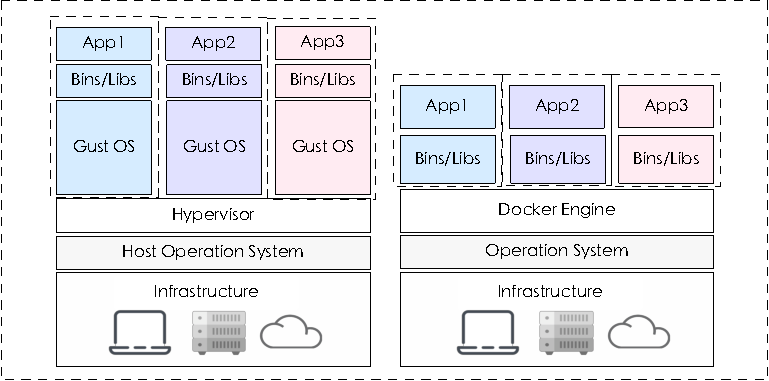
\includegraphics{docker-structure}
	\caption{容器与虚拟机对比}
	\label{fig:xfig1}
\end{figure}
图2-1中基础设施Infrastructure可以是个人电脑、服务器、云主机等,主机操作系统是运行在基础设施上的系统,最主要的是Linux各种版本,虚拟机管理系统(Hypervisor)可以实现在主机操作系统上独立运行多个子操作系统,在子操作系统上安装完应用所需的各种依赖后就可以实现资源应用的隔离。相对于虚拟机,Docker要简便很多,当前所有的Linux版本以及MacOS、Windows都能运行Docker,Docker Engine取代了Hypervisor,负载管理Docker容器并与操作系统通信,各种应用直接打包到镜像文件中,实现容器间的隔离。

对比Docker和虚拟机的架构发现,Docker直接通过守护进程与操作系统进行通信,管理容器并进行资源分配,实现容器与主操作系统的隔离。没有臃肿的子操作系统,各容器直接与主操作系统共享资源,节约了大量的磁盘空间,其虚拟化开销极大缩小,应用启动时间甚至达到毫秒级,用户可以快速构建、部署和交付应用,并且具有较强的跨平台性。
虽然Docker具有如此多的优势,但其隔离仅仅是在进程层面进行,并不能完全隔离整个运行环境。因此,用户需要根据自己的实际应用场景,需要彻底隔离用户的需求下选择虚拟机技术,如果仅是应用层面的隔离可以选择容器,如数据库、前端、后端等。
\subsection{OpenShift容器云平台}
\label{chap1:sample:table} 
Docker是当前主流的容器技术代表,Kubernetes作为现阶段应用最为广泛的容器编排引擎,OpenShift将这两种主流技术应用于企业,作为红帽公司提供的一款开源容器云平台。
该平台底层以Docker作为容器引擎驱动,Kubernetes作为容器编排组件,对外提供多种开发语言、中间件、数据库以及极易操作的用户界面、DevOps(Development and Operations)工具等。允许开发者和开发团队在该平台上进行应用的构建、测试、部署以及发布,是一套完整的容器应用云平台。在该平台上可以运行和支持有状态和无状态的应用;为容器应用提供较强的安全防护,包括基于用户的访问控制、检查机制以及强制隔离措施;实现多种综合云原生服务,便于快速智能、灵活开发应用、构建各种分布式系统;支持多种云环境包括Amazon Web Service、Azure、Google云平台以及VMware等;为开发运维团队提供一个通用的平台和工具,保持持续的开发和测试。OpenShift分为开源的社区版OpenShift Origin和收费的企业版OpenShift Enterprise,本文实验主要在开源的OpenShift Origin上进行分析和测试。
从技术堆栈的角度分析,OpenShift自下而上可以划分为基层架构层、容器引擎层、容器编排层、PaaS服务层、界面及工具层,如图2.2所示。下面分别对这几个层次进行介绍:
\begin{enumerate}[1.]
	\item 基础架构层。OpenShift运行所需的基础设施和环境,包括物理机、云主机、虚拟机、各种公有云、私有云以及混合云等。OpenShift支持多种操作系统,如CentOS7以上、Fedora21、Red Hat Enterprise Linux等,最后专门针对Atomic Host进行支持,是对企业版的Linux进行定制和优化的操作系统,可以为应用提供高度一致的运行环境,保证集群的稳定和安全。容器应用虽然具有较强的夸平台型,其前提是要求底层操作系统的内核和配置必须一致,因为其隔离依赖于Linux的内核。
	\item 容器引擎层。以当前主流的Docker作为OpenShift容器引擎,Docker已广泛应用于各种社区和环境中,经过了安全、稳定和高可用的检验。OpenShift并未修改任何原生的Docker代码,所有的应用最终到底层都生成一个Docker实例,只是将Docker的开放性和大量的镜像文件无缝衔接到平台上,对Docker的普通用户可以快速整合到平台中。
	\item 容器编排层。容器的编排对容器云的性能和资源利用效率具有决定性作用,OpenShift最终选择开源轻量的Kubernetes作为其容器编排引擎,Kubernetes已在Google内部使用多年,其诞生初衷就是为解决大规模集群中容器的调度和管理问题。OpenShift平台中很多基本的概念如Namespace、Pod、Replication Controller等都继承自Kubernetes,OpenShift同样只是将Kubernetes进行叠加使用,并未修改其原生代码和对象,用户依然可以通过原生的命令操作Kubernetes的对象。
	\item PaaS服务层。OpenShift在PaaS服务层提供了多种开发语言、框架、数据库以及中间件,极大提升了上层应用的开发、部署和交付速度。OpenShift有一个专门的社区以及Docker Hub提供各种应用的镜像,用户可以快速获取一个应用的基本镜像,构建自己所需的环,Red Hat的JBoss中间件几乎全部实现了容器化。
	\item 界面及工具层。OpenShift平台强大的界面及工具极大帮助普通用户高效完成相关应用业务,用户可以通过Web进行鼠标操作,平台将自动从Docker Hub中拉取所需的镜像进行应用构建,全自动化的服务极大降低了运维成本和提升服务效率。此外,OpenShift平台还提供S2I(Source to Image)服务,用户开发完成后可以自动整合到镜像中,快速实现交付,提升开发、测试、部署效率。针对用户端接入问题,平台提供Web控制台、IDE集成、命令行工具、以及RESTful API编程接口,用户可以最大限度的自由发挥。
\end{enumerate}
\begin{figure}[H] % use float package if you want it here
	\centering
	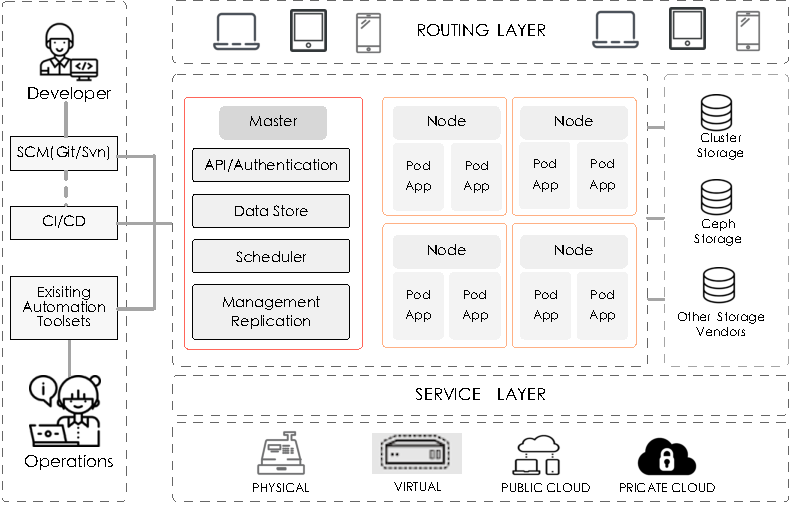
\includegraphics{openshift-structure}
	\caption{OpenShift Origin架构图}
	\label{fig:xfig1}
\end{figure}

如图2.2所示,OpenShift平台的核心组件包括Master、Node、Pod、Scheduler、Service、Storage等。Mater是主控节点,可以配置高可用的多个主控节点,负责管理和维护OpenShift集群的状态。Master上运行的API Server是其核心组件,所有用户的Web Console以及RESTful API服务都通过该组件进行访问认证控制,各Node节点也会定期轮询API Server更新其状态和容器的状态。Data Store将所有的状态信息存储在分布式的数据库Etcd中,并通过ceph一致性协议保证其数据的一致性,Etcd可以安装在主控节点,也可以单独安装到集群之外。Scheduler调度控制器进行Pod资源的分配和调度,收集过各节点资源情况,选择最优的节点作为容器应用的调度目标。Replication Controller异常自检测和恢复组件,负责监控集群中容器应用的状态和数量是否和用户要求一致,自启动和关闭容器应用满足用户的需求。Node节点通过接收Master节点指令维护容器应用。Pod是OpenShift平台调度器调度的最小单元,一些容器应用和应用之间往往存在较大的关联性,将几个联系紧密的容器部署在一个Pod中进行调度,提升应用的效率,如分布式数据库。容器是一个非持久化的对象,一旦容器重启或销毁,其状态信息将会随之销毁,集群每次给Pod分配的IP地址不同,要对外提供统一持久的服务,需要Service组件,该组件能将所有的信息转发到其对应的容器IP和端口上。此外,还有Router、Persistent Storage、Registry、Haproxy、Kubelet等都是集群的重要组成组件。数据的持久化存储可以是集群的数据库、分布式数据库或者其他的数据库中,当前支持的有NFS、Ceph RDB、GlusterFS等。
\section{定理环境}
\label{sec:theorem}

给大家演示一下各种和证明有关的环境:

\begin{assumption}
待月西厢下,迎风户半开;隔墙花影动,疑是玉人来。
\begin{eqnarray}
  \label{eq:eqnxmp}
  c & = & a^2 - b^2\\
    & = & (a+b)(a-b)
\end{eqnarray}
\end{assumption}

千辛万苦,历尽艰难,得有今日。然相从数千里,未曾哀戚。今将渡江,方图百年欢笑,如
何反起悲伤?(引自《杜十娘怒沉百宝箱》)

\begin{definition}
子曰:「道千乘之国,敬事而信,节用而爱人,使民以时。」
\end{definition}

千古第一定义!问世间、情为何物,只教生死相许?天南地北双飞客,老翅几回寒暑。欢乐趣,离别苦,就中更有痴儿女。
君应有语,渺万里层云,千山暮雪,只影向谁去?

横汾路,寂寞当年箫鼓,荒烟依旧平楚。招魂楚些何嗟及,山鬼暗谛风雨。天也妒,未信与,莺儿燕子俱黄土。
千秋万古,为留待骚人,狂歌痛饮,来访雁丘处。

\begin{proposition}
 曾子曰:「吾日三省吾身 —— 为人谋而不忠乎?与朋友交而不信乎?传不习乎?」
\end{proposition}

多么凄美的命题啊!其日牛马嘶,新妇入青庐,奄奄黄昏后,寂寂人定初,我命绝今日,
魂去尸长留,揽裙脱丝履,举身赴清池,府吏闻此事,心知长别离,徘徊庭树下,自挂东南
枝。

\begin{remark}
天不言自高,水不言自流。
\begin{gather*}
\begin{split} 
\varphi(x,z)
&=z-\gamma_{10}x-\gamma_{mn}x^mz^n\\
&=z-Mr^{-1}x-Mr^{-(m+n)}x^mz^n
\end{split}\\[6pt]
\begin{align} \zeta^0&=(\xi^0)^2,\\
\zeta^1 &=\xi^0\xi^1,\\
\zeta^2 &=(\xi^1)^2,
\end{align}
\end{gather*}
\end{remark}

天尊地卑,乾坤定矣。卑高以陈,贵贱位矣。 动静有常,刚柔断矣。方以类聚,物以群分,
吉凶生矣。在天成象,在地成形,变化见矣。鼓之以雷霆,润之以风雨,日月运行,一寒一
暑,乾道成男,坤道成女。乾知大始,坤作成物。乾以易知,坤以简能。易则易知,简则易
从。易知则有亲,易从则有功。有亲则可久,有功则可大。可久则贤人之德,可大则贤人之
业。易简,而天下矣之理矣;天下之理得,而成位乎其中矣。

\begin{axiom}
两点间直线段距离最短。  
\begin{align}
x&\equiv y+1\pmod{m^2}\\
x&\equiv y+1\mod{m^2}\\
x&\equiv y+1\pod{m^2}
\end{align}
\end{axiom}

《彖曰》:大哉乾元,万物资始,乃统天。云行雨施,品物流形。大明始终,六位时成,时
乘六龙以御天。乾道变化,各正性命,保合大和,乃利贞。首出庶物,万国咸宁。

《象曰》:天行健,君子以自强不息。潜龙勿用,阳在下也。见龙再田,德施普也。终日乾
乾,反复道也。或跃在渊,进无咎也。飞龙在天,大人造也。亢龙有悔,盈不可久也。用九,
天德不可为首也。   

\begin{lemma}
《猫和老鼠》是我最爱看的动画片。
\begin{multline*}%\tag*{[a]} % 这个不出现在索引中
\int_a^b\biggl\{\int_a^b[f(x)^2g(y)^2+f(y)^2g(x)^2]
 -2f(x)g(x)f(y)g(y)\,dx\biggr\}\,dy \\
 =\int_a^b\biggl\{g(y)^2\int_a^bf^2+f(y)^2
  \int_a^b g^2-2f(y)g(y)\int_a^b fg\biggr\}\,dy
\end{multline*}
\end{lemma}

行行重行行,与君生别离。相去万余里,各在天一涯。道路阻且长,会面安可知。胡马依北
风,越鸟巢南枝。相去日已远,衣带日已缓。浮云蔽白日,游子不顾返。思君令人老,岁月
忽已晚。  弃捐勿复道,努力加餐饭。

\begin{theorem}\label{the:theorem1}
犯我强汉者,虽远必诛\hfill —— 陈汤(汉)
\end{theorem}
\begin{subequations}
\begin{align}
y & = 1 \\
y & = 0
\end{align}
\end{subequations}
道可道,非常道。名可名,非常名。无名天地之始;有名万物之母。故常无,欲以观其妙;
常有,欲以观其徼。此两者,同出而异名,同谓之玄。玄之又玄,众妙之门。上善若水。水
善利万物而不争,处众人之所恶,故几于道。曲则全,枉则直,洼则盈,敝则新,少则多,
多则惑。人法地,地法天,天法道,道法自然。知人者智,自知者明。胜人者有力,自胜
者强。知足者富。强行者有志。不失其所者久。死而不亡者寿。

\begin{proof}
燕赵古称多感慨悲歌之士。董生举进士,连不得志于有司,怀抱利器,郁郁适兹土,吾
知其必有合也。董生勉乎哉?

夫以子之不遇时,苟慕义强仁者,皆爱惜焉,矧燕、赵之士出乎其性者哉!然吾尝闻
风俗与化移易,吾恶知其今不异于古所云邪?聊以吾子之行卜之也。董生勉乎哉?

吾因子有所感矣。为我吊望诸君之墓,而观于其市,复有昔时屠狗者乎?为我谢
曰:“明天子在上,可以出而仕矣!” \hfill —— 韩愈《送董邵南序》
\end{proof}

\begin{corollary}
  四川话配音的《猫和老鼠》是世界上最好看最好听最有趣的动画片。
\begin{alignat}{3}
V_i & =v_i - q_i v_j, & \qquad X_i & = x_i - q_i x_j,
 & \qquad U_i & = u_i,
 \qquad \text{for $i\ne j$;}\label{eq:B}\\
V_j & = v_j, & \qquad X_j & = x_j,
  & \qquad U_j & u_j + \sum_{i\ne j} q_i u_i.
\end{alignat}
\end{corollary}

迢迢牵牛星,皎皎河汉女。
纤纤擢素手,札札弄机杼。
终日不成章,泣涕零如雨。
河汉清且浅,相去复几许。
盈盈一水间,脉脉不得语。

\begin{example}
  大家来看这个例子。
\begin{equation}
\label{ktc}
\left\{\begin{array}{l}
\nabla f({\mbox{\boldmath $x$}}^*)-\sum\limits_{j=1}^p\lambda_j\nabla g_j({\mbox{\boldmath $x$}}^*)=0\\[0.3cm]
\lambda_jg_j({\mbox{\boldmath $x$}}^*)=0,\quad j=1,2,\cdots,p\\[0.2cm]
\lambda_j\ge 0,\quad j=1,2,\cdots,p.
\end{array}\right.
\end{equation}
\end{example}

\begin{exercise}
  请列出 Andrew S. Tanenbaum 和 W. Richard Stevens 的所有著作。
\end{exercise}

\begin{conjecture} \textit{Poincare Conjecture} If in a closed three-dimensional
  space, any closed curves can shrink to a point continuously, this space can be
  deformed to a sphere.
\end{conjecture}

\begin{problem}
 回答还是不回答,是个问题。 
\end{problem}

如何引用定理~\ref{the:theorem1} 呢?加上 \cs{label} 使用 \cs{ref} 即可。妾发
初覆额,折花门前剧。郎骑竹马来,绕床弄青梅。同居长干里,两小无嫌猜。 十四为君妇,
羞颜未尝开。低头向暗壁,千唤不一回。十五始展眉,愿同尘与灰。常存抱柱信,岂上望夫
台。 十六君远行,瞿塘滟滪堆。五月不可触,猿声天上哀。门前迟行迹,一一生绿苔。苔深
不能扫,落叶秋风早。八月蝴蝶来,双飞西园草。感此伤妾心,坐愁红颜老。

\section{参考文献}
\label{sec:bib}
当然参考文献可以直接写 \cs{bibitem},虽然费点功夫,但是好控制,各种格式可以自己随意改
写。

本模板推荐使用 BIB\TeX,分别提供数字引用(\texttt{thuthesis-numeric.bst})和作
者年份引用(\texttt{thuthesis-author-year.bst})样式,基本符合学校的参考文献格式
(如专利等引用未加详细测试)。看看这个例子,关于书的~\cite{tex, companion,
  ColdSources},还有这些~\cite{Krasnogor2004e, clzs, zjsw},关于杂志
的~\cite{ELIDRISSI94, MELLINGER96, SHELL02},硕士论文~\cite{zhubajie,
  metamori2004},博士论文~\cite{shaheshang, FistSystem01},标准文
件~\cite{IEEE-1363},会议论文~\cite{DPMG,kocher99},技术报告~\cite{NPB2},电子文
献~\cite{chuban2001,oclc2000}。中文参考文献~\cite{cnarticle}应增
加 \texttt{language=``chinese''} 字段,以便进行相应处理。另外,本模板对中文文
献~\cite{cnproceed}的支持并不是十全十美,如果有不如意的地方,请手动修
改 \texttt{bbl} 文件。

有时候不想要上标,那么可以这样~\inlinecite{shaheshang},这个非常重要。

有时候一些参考文献没有纸质出处,需要标注 URL。缺省情况下,URL 不会在连字符处断行,
这可能使得用连字符代替空格的网址分行很难看。如果需要,可以将模板类文件中
\begin{verbatim}
\RequirePackage{hyperref}
\end{verbatim}
一行改为:
\begin{verbatim}
\PassOptionsToPackage{hyphens}{url}
\RequirePackage{hyperref}
\end{verbatim}
使得连字符处可以断行。更多设置可以参考 \texttt{url} 宏包文档。

\section{公式}
\label{sec:equation}
贝叶斯公式如式~(\ref{equ:chap1:bayes}),其中 $p(y|\mathbf{x})$ 为后验;
$p(\mathbf{x})$ 为先验;分母 $p(\mathbf{x})$ 为归一化因子。
\begin{equation}
\label{equ:chap1:bayes}
p(y|\mathbf{x}) = \frac{p(\mathbf{x},y)}{p(\mathbf{x})}=
\frac{p(\mathbf{x}|y)p(y)}{p(\mathbf{x})} 
\end{equation}

论文里面公式越多,\TeX{} 就越 happy。再看一个 \pkg{amsmath} 的例子:
\newcommand{\envert}[1]{\left\lvert#1\right\rvert} 
\begin{equation}\label{detK2}
\det\mathbf{K}(t=1,t_1,\dots,t_n)=\sum_{I\in\mathbf{n}}(-1)^{\envert{I}}
\prod_{i\in I}t_i\prod_{j\in I}(D_j+\lambda_jt_j)\det\mathbf{A}
^{(\lambda)}(\overline{I}|\overline{I})=0.
\end{equation} 

前面定理示例部分列举了很多公式环境,可以说把常见的情况都覆盖了,大家在写公式的时
候一定要好好看 \pkg{amsmath} 的文档,并参考模板中的用法:
\begin{multline*}%\tag{[b]} % 这个出现在索引中的
\int_a^b\biggl\{\int_a^b[f(x)^2g(y)^2+f(y)^2g(x)^2]
 -2f(x)g(x)f(y)g(y)\,dx\biggr\}\,dy \\
 =\int_a^b\biggl\{g(y)^2\int_a^bf^2+f(y)^2
  \int_a^b g^2-2f(y)g(y)\int_a^b fg\biggr\}\,dy
\end{multline*}

其实还可以看看这个多级规划:
\begin{equation}\label{bilevel}
\left\{\begin{array}{l}
\max\limits_{{\mbox{\footnotesize\boldmath $x$}}} F(x,y_1^*,y_2^*,\cdots,y_m^*)\\[0.2cm]
\mbox{subject to:}\\[0.1cm]
\qquad G(x)\le 0\\[0.1cm]
\qquad(y_1^*,y_2^*,\cdots,y_m^*)\mbox{ solves problems }(i=1,2,\cdots,m)\\[0.1cm]
\qquad\left\{\begin{array}{l}
    \max\limits_{{\mbox{\footnotesize\boldmath $y_i$}}}f_i(x,y_1,y_2,\cdots,y_m)\\[0.2cm]
    \mbox{subject to:}\\[0.1cm]
    \qquad g_i(x,y_1,y_2,\cdots,y_m)\le 0.
    \end{array}\right.
\end{array}\right.
\end{equation}
这些跟规划相关的公式都来自于刘宝碇老师《不确定规划》的课件。
